%%!TEX TS-program = latex
\documentclass{beamer}
\usepackage{etex}
\usepackage{booktabs}
\reserveinserts{20}
\usepackage{latexsym}
\usepackage{amsmath}
\usepackage{amssymb}
\usepackage{transparent}
\usepackage{tikz,etoolbox}
\usepackage{tikz,amsmath,siunitx}
\usetikzlibrary{arrows,snakes,backgrounds,patterns,matrix,shapes,fit,calc,shadows,plotmarks}
% set \pdfoutput to 0 for .dvi, or 1 for .pdf output
% \pdfoutput=0


\usepackage{beamerthemeshadow}
\usepackage{color}
\usepackage{multirow}
\usepackage{rotating}
\usepackage[all,dvips]{xy}
\usepackage{colortbl}
\usepackage{graphicx}
\usepackage{verbatim}
\usepackage{framed}
\usepackage{natbib}
\usepackage[labelformat=empty]{caption}
\usepackage{colortbl}
%\usepackage{fancybox}
% \usepackage{amsmath,amsthm}
%\usepackage{graphics}
%\input{epsf}
%\usepackage[ps,dvips,all]{xy}
%\usepackage[all]{xy}

\usepackage{algorithm}
\usepackage{algpseudocode}
\usepackage{comment}
\usepackage[normalem]{ulem}
\newcommand\tst{% thick strike through  %% from http://tex.stackexchange.com/questions/134088/mis-alignment-of-columns-in-tabular-environment-when-using-ulem-and-beamer
  \bgroup%
  \markoverwith{\textcolor{red}{\rule[1.1ex]{1pt}{0.8pt}}}%
  \ULon%
}

\algtext*{EndWhile}% Remove "end while" text
\algtext*{EndFor}% Remove "end while" text
\algtext*{EndIf}% Remove "end if" text
\algtext*{EndProcedure}% Remove "end while" text

\setbeamertemplate{navigation symbols}{}%remove navigation symbols
\renewcommand{\rmdefault}{crm}
\newcommand{\lnbrack}{{\normalfont [}}
\newcommand{\rnbrack}{{\normalfont ]}\thinspace}
\newcommand{\lbbrack}{\textcolor{red}{\textbf{[}}}
\newcommand{\rbbrack}{\textcolor{red}{\textbf{]}}\thinspace}
\newcommand{\air}{\vspace{0.25cm}}
\newcommand{\mair}{\vspace{-0.25cm}}


\def\printlandscape{\special{landscape}}

% rgb values are divided by 255
%\definecolor{Gold}{rgb}{0.62, 0.5, 0.22}
%\definecolor{Crimson}{HTML}{AD1022}
\definecolor{Crimson}{RGB}{165, 28, 48}	

% i'm defining some colors that are supposed to be easy for colorblind people to distinguish. see http://jfly.iam.u-tokyo.ac.jp/color/index.html#select
\definecolor{orange}{RGB}{230,159,0}
\definecolor{skyblue}{RGB}{86,180,233}
\definecolor{bluegreen}{RGB}{0,158,115}
\definecolor{myyellow}{RGB}{240,228,66} % i dunno if this is the same as standard yellow
\definecolor{myblue}{RGB}{0,114,178}
\definecolor{vermillion}{RGB}{213,94,0}
\definecolor{redpurple}{RGB}{204,121,167}
\definecolor{lightgrey}{RGB}{234,234,234}
\definecolor{Gray}{gray}{0.9}

%\setbeamercolor{footlinecolor}{fg=white,bg=black}

\setbeamercolor{lowercol}{fg=black,bg=structure!25}%
% \setbeamercolor{lowercol}{fg=black,bg=WarmGray}%
\newenvironment{researchquestion}
{\begin{beamerboxesrounded} [lower=lowercol,shadow=true]{}}
{\end{beamerboxesrounded}}
%\setbeamercolor{block body}{bg=lightgrey}

\newcommand{\given}{\,|\,}
\newcommand{\Cite}[1]{{\footnotesize\cite{#1}}}
\newcommand{\TT}[1]{{\footnotesize\tt{#1}}}
\newcommand{\boldw}{\boldsymbol{w}}
\newcommand{\boldu}{\boldsymbol{u}}
\newcommand{\boldv}{\boldsymbol{v}}
\newcommand{\boldb}{\boldsymbol{b}}
\newcommand{\boldW}{\boldsymbol{W}}
\newcommand{\boldh}{\boldsymbol{h}}
\newcommand{\boldg}{\boldsymbol{g}}
\newcommand{\boldz}{\boldsymbol{z}}
\newcommand{\boldq}{\boldsymbol{q}}
\newcommand{\boldm}{\boldsymbol{m}}
\newcommand{\boldx}{\boldsymbol{x}}
\newcommand{\boldy}{\boldsymbol{y}}
\newcommand{\bzero}{\boldsymbol{0}}
%\newcommand{\bphi}{\ensuremath{\mathbf{\phi}}}
\newcommand{\bphi}{\boldsymbol{\phi}}
\newcommand{\btheta}{\boldsymbol{\theta}}
\newcommand{\mcY}{\mathcal{Y}}
\newcommand{\mcX}{\mathcal{X}}
\newcommand{\mcC}{\mathcal{C}}
\newcommand{\mcA}{\mathcal{A}}
\newcommand{\mcV}{\mathcal{V}}
\newcommand{\mcL}{\mathcal{L}}
\newcommand{\trans}{\ensuremath{\mathsf{T}}}
\def\argmin{\operatornamewithlimits{arg\,min}}
\def\argmax{\operatornamewithlimits{arg\,max}}
\newcommand{\reals}{\ensuremath{\mathbb{R}}}
\newcommand{\RNN}{\mathrm{RNN}}
\newcommand{\BRNN}{\mathrm{BRNN}}

\newcommand{\clust}{\ensuremath{\mathrm{clust}}}
\newcommand{\loc}{\ensuremath{\mathrm{loc}}}
\newcommand{\nicein}{\ensuremath{\,{\in}\,}}
\newcommand{\niceq}{\ensuremath{\,{=}\,}}
\newcommand{\uc}{\ensuremath{\mathrm{c}}}
\newcommand{\hc}{\boldh_{\uc}}
\newcommand{\cb}{\boldb_{\mathrm{\uc}}}
\newcommand{\cW}{\boldW_{\mathrm{\uc}}}

\newcommand{\aphi}{\boldsymbol{\phi}_{\mathrm{a}}}
\newcommand{\pwphi}{\boldsymbol{\phi}_{\mathrm{p}}}
\newcommand{\squigaphi}{\widetilde{\boldsymbol{\phi}}_{\mathrm{a}}}
\newcommand{\squigpwphi}{\widetilde{\boldsymbol{\phi}}_{\mathrm{p}}}

\newcommand{\aW}{\boldW_{\mathrm{\ua}}}
\newcommand{\pW}{\boldW_{\mathrm{\up}}}

\newcommand{\ab}{\boldb_{\mathrm{\ua}}}
\newcommand{\pb}{\boldb_{\mathrm{\up}}}

\newcommand{\Da}{d_{\mathrm{a}}}
\newcommand{\Dp}{d_{\mathrm{p}}}

\newcommand{\ha}{\boldh_{\ua}}
\newcommand{\hp}{\boldh_{\up}}

\newcommand{\ourmodel}{This work}
\newcommand{\zro}{{\color{white}0}}
\newcommand{\fix}[1]{{\color{white}1}#1}
\newcommand{\fixg}[1]{{\color{Gray}1}#1}

\newcommand{\enc}{\mathrm{src}}
\newcommand{\xvec}{\mathbf{x}}
\newcommand{\yvec}{\mathbf{y}}
\newcommand{\wvec}{\mathbf{w}}
\newcommand{\cvec}{\mathbf{c}}
\newcommand{\zvec}{\mathbf{z}}
% \newcommand{\mcY}{\mathcal{Y}}
% \newcommand{\mcV}{\mathcal{V}}
\newcommand{\context}{\mathbf{w}_{\mathrm{c}}}
\newcommand{\embcontext}{\mathbf{\tilde{w}}_{\mathrm{c}}}
\newcommand{\inpcontext}{\mathbf{\tilde{x}}}
\newcommand{\start}{\mathbf{\tilde{y}}_{\mathrm{c0}}}
\newcommand{\End}{\mathrm{\texttt{</s>}}}

\newcommand{\Uvec}{\mathbf{U}}
\newcommand{\Evec}{\mathbf{E}}
\newcommand{\Gvec}{\mathbf{G}}
\newcommand{\Fvec}{\mathbf{F}}
\newcommand{\Pvec}{\mathbf{P}}
\newcommand{\pvec}{\mathbf{p}}
\newcommand{\Qvec}{\mathbf{Q}}
\newcommand{\Vvec}{\mathbf{V}}
\newcommand{\Wvec}{\mathbf{W}}
\newcommand{\hvec}{\mathbf{h}}
\newcommand{\softmax}{\mathrm{softmax}}
% \newcommand{\reals}{\mathbb{R}}


\def\argmin{\operatornamewithlimits{arg\,min}}
\def\argmax{\operatornamewithlimits{arg\,max}}


\def\argmax{\operatornamewithlimits{arg\,max}}
\def\kargmax{\operatornamewithlimits{K-arg\,max}}
%\DeclareMathOperator{\topK}{topK}
\def\topK{\operatornamewithlimits{topK}}
\DeclareMathOperator{\suk}{succ}
\newcommand{\longpfx}[1]{\ensuremath{w_1 \cdots w_{#1}}}
\newcommand{\longgoldpfx}[1]{\ensuremath{y_1 \cdots y_{#1}}}
\newcommand{\pfx}[1]{\ensuremath{w_{1:{#1}}}}
\newcommand{\goldpfx}[1]{\ensuremath{y_{1:{#1}}}}
\newcommand{\beampred}[2]{\ensuremath{\hat{y}_{1:{#1}}^{({#2})}}}

\usefonttheme{professionalfonts}

% http://www.tug.org/pracjourn/2005-4/mertz/mertz.pdf
% \setbeamertemplate{footline}[text line]{Predicting Events \hfill \thepage}
%\usefoottemplate{\vbox{{\color{white}{E.W. Fulp\hfill SIAM'09~} \insertshortdate  \insertframenumber/\inserttotalframenumber}}}
%\usefoottemplate{\vbox{{ \insertshortdate  \insertframenumber/\inserttotalframenumber}}}

%\setbeamertemplate{footline}[text line]{%
%\begin{beamercolorbox}[sep=1em, wd=\paperwidth, leftskip=.25cm, rightskip=.5cm]{footlinecolor}
%  \inserttitle \hfill\hfill\insertpagenumber
%\end{beamercolorbox}
%}
\setbeamertemplate{navigation symbols}{}
% \setbeamertemplate{bibliography item}[text]

% for handouts
\usepackage{pgfpages}
% \pgfpagesuselayout{2 on 1}[letterpaper,border shrink=5mm]
\pgfpagesuselayout{resize to}[letterpaper,border shrink=5mm,landscape]
% \pgfpagesuselayout{resize to}[letterpaper,landscape]


%Harvard Crimson
\setbeamercolor{structure}{fg=Crimson}

% \logo{\includegraphics[height=0.25cm]{WFU_Univ_H_Black.eps}}

\setbeamersize{text margin left=6mm}
\setbeamersize{text margin right=6mm}
\renewcommand{\insertnavigation}[1]{}
\setbeamertemplate{headline}{}
\setbeamertemplate{footline}{}
% make itemize things larger
%\setbeamerfont*{itemize/enumerate body}{size=\Large}
%\setbeamerfont*{itemize/enumerate subbody}{size=\large}
\setbeamercovered{transparent}
\mode<presentation>
%\mode<handout>
\linespread{1.25}

%citation stuff
\let\realcitep\citep
\renewcommand*{\citep}[1]{{\footnotesize \realcitep{#1}}}
\setcitestyle{square,semicolon,aysep={}} 

% \def\thefootnote{\fnsymbol{footnote}}

%\renewcommand<>{\sout}[1]{
%  \alt#2{\beameroriginal{\sout}{#1}}{#1}
%}

\title{Sequence-to-Sequence Learning\\ as Beam-Search Optimization}
% width=36mm
\institute{
\centering
\includegraphics[scale=0.3]{SEASLogo.png} 
}
\author{Sam Wiseman and Alexander M. Rush}
             
\date{}

\def\signed #1{{\leavevmode\unskip\nobreak\hfil\penalty50\hskip2em
  \hbox{}\nobreak\hfil(#1)%
  \parfillskip=0pt \finalhyphendemerits=0 \endgraf}}

\newsavebox\mybox
\newenvironment{aquote}[1]
  {\savebox\mybox{#1}\begin{quote}}
  {\signed{\usebox\mybox}\end{quote}}



\begin{document}

\begin{frame}
	\maketitle
\end{frame}

\begin{frame}
    \frametitle{Seq2Seq as a General-purpose NLP/Text Generation Tool}

  \begin{itemize}
  \item Machine Translation \Cite{kalchbrenner2013recurrent,sutskever2014sequence, Cho2014, bahdanau2014neural,luong15effective} 
  \item Question Answering \Cite{Hermann2015} 
  \item Conversation \Cite{Vinyals2015}
  \item Parsing \Cite{vinyals15grammar}
  %\item Argument Generation \Cite{Wang}
  \item Sentence Compression \Cite{filippova15sentence}
  %\item Speech \Cite{Chorowski2015}
  \item Summarization \Cite{Rush2015} 
  \item Caption Generation \Cite{Xu2015}
  \item Video-to-Text \Cite{Venugopalan2015}
  \item Grammar Correction \Cite{Schmaltz2016}
  \end{itemize}
  
\end{frame}

\begin{frame}
\frametitle{Room for Improvement?}
Despite its tremendous success, there are some potential issues with standard Seq2Seq~\citep{ranzato16sequence,bengio15scheduled}:

\begin{itemize}
\air
\item[(1)] Train/Test mismatch
\air
\item[(2)] Seq2Seq models next-words, rather than whole sequences
\end{itemize}

\air
\air
\textbf{Goal of the talk}: describe a simple variant of Seq2Seq --- and corresponding beam-search training scheme --- to address these issues.
%\begin{itemize}
%\item Unifies training and test
%\item Models at the sequence level
%\item Doesn't require RL! 
%\end{itemize}


\end{frame}

\begin{frame}[t]
\frametitle{Review: Sequence-to-sequence (Seq2Seq) Models}

    \begin{center}
      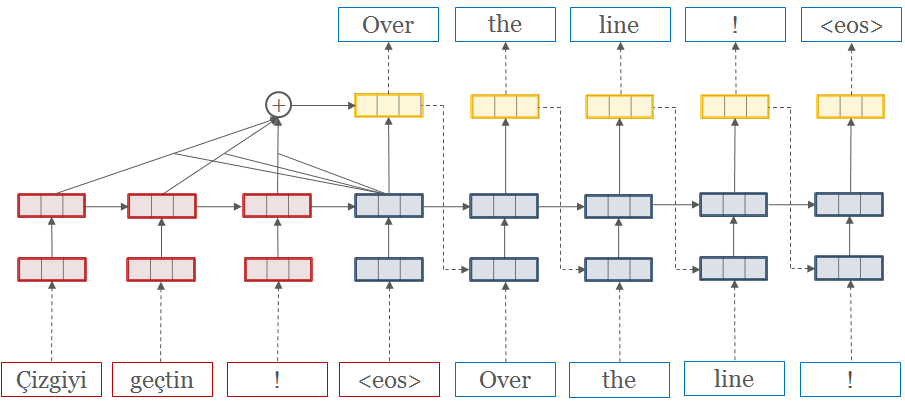
\includegraphics[width=0.7\textwidth]{simple-attn}
    \end{center}

\air
\air    
\begin{itemize}
\item Encoder RNN (red) encodes source into a representation $\boldx$
\air
\item Decoder RNN (blue) generates translation word-by-word
\end{itemize}
\end{frame}

\begin{frame}
\frametitle{Review: Seq2Seq Generation Details}
\begin{center}
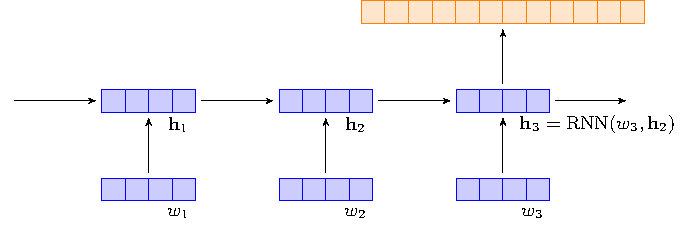
\includegraphics[scale=0.8]{rnntikzpicz/rnnlm}
\end{center}

\begin{itemize}

\item Probability of generating $t$'th word: 
\begin{align*}
p(w_t | w_1, \ldots, w_{t-1}, \boldx ; \theta) = \softmax(\mathbf{W}_{out} \, \mathbf{h}_{t-1} + \mathbf{b}_{out})
\end{align*}
\end{itemize}
\end{frame}

%\begin{frame}
%\frametitle{Do we really need this?}
%We have $\boldx_1,\ldots,\boldx_n$ and $\boldy = y_1,\ldots, y_T$
%\end{frame}

\begin{frame}
  \frametitle{Review: Train and Test}

  \textbf{Train Objective}: Given source-target pairs $(x, y_{1:T})$, minimize NLL of each word independently, conditioned on \textit{gold} history $y_{1:t-1}$
\begin{align*}
\text{NLL}(\theta) = -\sum_{t} \ln p(w_{t} = y_t | y_{1:t-1}, \boldx; \theta) 
\end{align*}

  \air

\textbf{Test Objective}:  Structured prediction
  \begin{align*}
  \hat{y}_{1:T} = \argmax_{w_{1:T}} \sum_{t} \ln p(w_{t} | w_{1:t-1}, \boldx; \theta)
\end{align*}
\begin{itemize}
\item Typical to approximate the $\argmax$ with beam-search
\end{itemize}
\end{frame}

%\begin{frame}[fragile]
%\frametitle{Beam Search Example ($K=3$)}
%    \begin{center}
%  \begin{tikzpicture}[transform canvas = {scale=0.8}]
%    \tikzstyle{beam}=[draw, minimum height=0.6cm, anchor=base, text height=5, text depth=0, minimum width=1.5cm,thin, rounded corners, line width=0.03cm]
%   \tikzstyle{mat}=[draw=white]
%    \tikzset{>=stealth',every on chain/.append style={join},
%      every join/.style={->}}
%
%     
%       \begin{scope}
%         
%   \matrix (G) [matrix of nodes, nodes={beam},inner sep=1mm,row sep=0.03cm, column sep=0.8cm ] {
%    \node<1->(G-1-1){a}; & \node<2->(G-1-2){red}; & \node<3->(G-1-3){dog}; & \node<4->(G-1-4){smells}; & \node<5->(G-1-5){home};  & \node<6->(G-1-6){today}; \\
%    \node<1->(G-2-1){the}; & \node<2->(G-2-2){dog}; & \node<3->(G-2-3){dog}; & \node<4->(G-2-4){barks}; & \node<5->(G-2-5){quickly}; & \node<6->(G-2-6){Friday}; \\
%    \node<1->(G-3-1){red}; & \node<2->(G-3-2){blue}; & \node<3->(G-3-3){cat}; &  \node<4->(G-3-4){walks}; & \node<5->(G-3-5){straight}; & \node<6->(G-3-6){now}; \\    };
%
%    \only<2->{
%      \draw[->] (G-1-1.east) -> (G-1-2.west); 
%      \draw[->] (G-2-1.east) -> (G-2-2.west); 
%      \draw[->] (G-1-1.east) -> (G-3-2.west); 
%      \draw[double, line width=0.03cm] (G-3-1.south west) -- (G-3-2.south east);
%    }
%  
%    \only<3->{
%      \draw[->] (G-1-2.east) -> (G-2-3.west); 
%      \draw[->] (G-3-2.east) -> (G-3-3.west); 
%      \draw[->] (G-3-2.east) -> (G-1-3.west); 
%      \draw[double, line width=0.03cm] (G-3-1.south west) -- (G-3-3.south east);
%    }
%    
% \only<4->{
%    \draw[->] (G-1-3.east) -> (G-3-4.west); 
%    \draw[->] (G-2-3.east) -> (G-2-4.west); 
%    \draw[->] (G-1-3.east) -> (G-1-4.west); 
%    \draw[double, line width=0.03cm] (G-3-1.south west) -- (G-3-4.south east);
%}
% \only<6->{
%    \draw[->] (G-1-5.east) -> (G-1-6.west); 
%    \draw[->] (G-1-5.east) -> (G-3-6.west); 
%    \draw[->] (G-2-5.east) -> (G-2-6.west); 
%    \draw[double, line width=0.03cm] (G-3-1.south west) -- (G-3-6.south east);
%}
%
% \only<5->{
%    \draw[->] (G-3-4.east) -> (G-1-5.west); 
%    \draw[->] (G-3-4.east) -> (G-2-5.west); 
%    \draw[->] (G-3-4.east) -> (G-3-5.west); 
%    \draw[double, line width=0.03cm] (G-3-1.south west) -- (G-3-5.south east);
%}
%
%\end{scope}
%\end{tikzpicture}
%\end{center}
%
%    \air
%    \air
%    \air
%For $t \niceq 1 \ldots T$:
%   \begin{itemize}
%   \item For all $k$ and for all possible output words $w$:
%     \begin{align*}
%     s(w_t \niceq w, \hat{y}_{1:t-1}^{(k)}) \gets \ln p(\hat{y}^{(k)}_{1:t-1}| \boldx) + \ln p(w_{t} \niceq w | \hat{y}^{(k)}_{1:t-1}, \boldx) \end{align*}
%   \item Update beam:
%%     \begin{align*}
%%     \hspace*{-4.4cm} \hat{y}_{1:t}^{(1:K)} \gets \topK_{s} \left\lbrace \mcV \times \hat{y}_{1:t-1}^{(1:K)} \right\rbrace
%%\end{align*}  
%\begin{align*}
%\hspace*{-4cm} \hat{y}_{1:t}^{(1:K)} \gets \kargmax_{w_{1:t}} \, s(w_t, \hat{y}_{1:t-1}^{(k)})
%\end{align*}
%   \end{itemize}
%\end{frame}

%\begin{frame}[fragile]
%\frametitle{Beam Search Example ($K=3$)}
%    \begin{center}
%
%\end{center}
%
%    \air
%    \air
%    \air
%For $t \niceq 1 \ldots T$:
%   \begin{itemize}
%   \item For all $k$ and for all possible output words $w$:
%     \begin{align*}
%     {s(w_t \niceq w, \hat{y}_{1:t-1}^{(k)})} \gets {\ln p(\hat{y}^{(k)}_{1:t-1}| \boldx)} + {\ln p(w_{t} \niceq w | \hat{y}^{(k)}_{1:t-1}, \boldx)} \end{align*}
%   \item Update beam:
%%     \begin{align*}
%%     \hspace*{-4.4cm} \hat{y}_{1:t}^{(1:K)} \gets \topK_{s} \left\lbrace \mcV \times \hat{y}_{1:t-1}^{(1:K)} \right\rbrace
%%\end{align*}  
%\begin{align*}
%\hspace*{-4cm} {\hat{y}_{1:t}^{(1:K)}} \gets {\kargmax_{w_{1:t}}} \, s(w_t, \hat{y}_{1:t-1}^{(k)})
%\end{align*}
%   \end{itemize}
%\end{frame}

\begin{frame}[fragile]
\frametitle{Review: Beam Search at Test Time ($K=3$)}
    \begin{center}
  \begin{tikzpicture}[transform canvas = {scale=0.8}]
    \tikzstyle{beam}=[draw, minimum height=0.6cm, anchor=base, text height=5, text depth=0, minimum width=1.5cm,thin, rounded corners, line width=0.03cm]
   \tikzstyle{mat}=[draw=white]
    \tikzset{>=stealth',every on chain/.append style={join},
      every join/.style={->}}

     
       \begin{scope}
         
   \matrix (G) [matrix of nodes, nodes={beam},inner sep=1mm,row sep=0.03cm, column sep=0.8cm ] {
    \node<1->(G-1-1){a}; & \node<7->(G-1-2){red}; & \node<8->(G-1-3){dog}; & \node<9->(G-1-4){smells}; & \node<10->(G-1-5){home};  & \node<11->(G-1-6){today}; \\
    \node<1->(G-2-1){the}; & \node<7->(G-2-2){dog}; & \node<8->(G-2-3){dog}; & \node<9->(G-2-4){barks}; & \node<10->(G-2-5){quickly}; & \node<11->(G-2-6){Friday}; \\
    \node<1->(G-3-1){red}; & \node<7->(G-3-2){blue}; & \node<8->(G-3-3){cat}; &  \node<9->(G-3-4){walks}; & \node<10->(G-3-5){straight}; & \node<11->(G-3-6){now}; \\    };

    \only<7->{
      \draw[->] (G-1-1.east) -> (G-1-2.west); 
      \draw[->] (G-2-1.east) -> (G-2-2.west); 
      \draw[->] (G-1-1.east) -> (G-3-2.west); 
      \draw[double, line width=0.03cm] (G-3-1.south west) -- (G-3-2.south east);
    }
  
    \only<8->{
      \draw[->] (G-1-2.east) -> (G-2-3.west); 
      \draw[->] (G-3-2.east) -> (G-3-3.west); 
      \draw[->] (G-3-2.east) -> (G-1-3.west); 
      \draw[double, line width=0.03cm] (G-3-1.south west) -- (G-3-3.south east);
    }
    
 \only<9->{
    \draw[->] (G-1-3.east) -> (G-3-4.west); 
    \draw[->] (G-2-3.east) -> (G-2-4.west); 
    \draw[->] (G-1-3.east) -> (G-1-4.west); 
    \draw[double, line width=0.03cm] (G-3-1.south west) -- (G-3-4.south east);
}
 \only<11->{
    \draw[->] (G-1-5.east) -> (G-1-6.west); 
    \draw[->] (G-1-5.east) -> (G-3-6.west); 
    \draw[->] (G-2-5.east) -> (G-2-6.west); 
    \draw[double, line width=0.03cm] (G-3-1.south west) -- (G-3-6.south east);
}

 \only<10->{
    \draw[->] (G-3-4.east) -> (G-1-5.west); 
    \draw[->] (G-3-4.east) -> (G-2-5.west); 
    \draw[->] (G-3-4.east) -> (G-3-5.west); 
    \draw[double, line width=0.03cm] (G-3-1.south west) -- (G-3-5.south east);
}

\end{scope}
\end{tikzpicture}
\end{center}

    \air
    \air
    \air
For $t \niceq 1 \ldots T$:
   \begin{itemize}
   \item For all $k$ and for all possible output words $w$:
     \begin{align*}
     \alert<2>{s(w_t \niceq w, \hat{y}_{1:t-1}^{(k)})} \gets \alert<3>{\ln p(\hat{y}^{(k)}_{1:t-1}| \boldx)} + \alert<4>{\ln p(w_{t} \niceq w | \hat{y}^{(k)}_{1:t-1}, \boldx)} \end{align*}
   \item Update beam:
%     \begin{align*}
%     \hspace*{-4.4cm} \hat{y}_{1:t}^{(1:K)} \gets \topK_{s} \left\lbrace \mcV \times \hat{y}_{1:t-1}^{(1:K)} \right\rbrace
%\end{align*}  
\begin{align*}
\hspace*{-4cm} \alert<5>{\hat{y}_{1:t}^{(1:K)}} \gets \alert<6>{\kargmax_{w_{1:t}}} \, s(w_t, \hat{y}_{1:t-1}^{(k)})
\end{align*}
   \end{itemize}
\end{frame}

\begin{frame}
\frametitle{Seq2Seq Issues Revisited}

\textbf{Issue \#1: Train/Test Mismatch} (cf., \Cite{ranzato16sequence})
\air
\begin{align*}
\text{NLL}(\theta) = -\sum_{t} \ln p(w_{t} = y_t | \alert<2>{y_{1:t-1}}, \boldx; \theta) 
\end{align*}

\begin{enumerate}
\pause
\item[(a)] Training conditions on \textit{true} history (``Exposure Bias'')
\pause
\item[(b)] Train with word-level NLL, but evaluate with BLEU-like metrics
\end{enumerate}


\air
\air
\air
\pause
\textbf{Idea \#1:} Train with beam-search
\air
\begin{itemize}
\item Use a loss that incorporates (sub)sequence-level costs
\end{itemize}


\end{frame}

\begin{frame}
\frametitle{Idea \#1: Train with Beam Search}
Replace NLL with loss that penalizes search-error: 
\begin{align*}
 \mathcal{L}&(\theta) = \sum_{t} \alert<4>{\Delta(\hat{y}_{1:t}^{(K)})} \left[1  - \alert<2>{s(y_t, y_{1:t-1})} +  \alert<3>{s(\hat{y}_t^{(K)}, \hat{y}_{1:t-1}^{(K)})} \right] 
\end{align*}

\begin{itemize}
\item $y_{1:t}$ is the gold prefix; $\hat{y}_{1:t}^{(K)}$ is the $K$'th prefix on the beam
\air
\air
\item $s(\hat{y}_t^{(k)}, \hat{y}_{1:t-1}^{(k)})$ is the score of history $(\hat{y}_t^{(k)}, \hat{y}_{1:t-1}^{(k)})$ 
\air 
\air
\item $\Delta(\hat{y}_{1:t}^{(K)})$ allows us to scale loss by badness of predicting $\hat{y}_{1:t}^{(K)}$
 
%\air
%\item Want gold on top at the end, so when $t \niceq T$, replace %$\hat{y}_{1:T}^{(K)}$ with highest-scoring incorrect sequence
\end{itemize}
\end{frame}


\begin{frame}
\frametitle{Seq2Seq Issues Revisited}

\textbf{Issue \#2: Seq2Seq models next-word probabilities}:
\air
\begin{align*}
\hspace*{-1cm} s(w_t \niceq w, \hat{y}_{1:t-1}^{(k)}) \gets \ln p(\hat{y}^{(k)}_{1:t-1}| \boldx) + \ln p(w_{t} \niceq w | \hat{y}^{(k)}_{1:t-1}, \boldx) 
\end{align*}

\begin{enumerate}
\pause
\item[(a)] Sequence score is sum of locally normalized word-scores; gives rise to ``Label Bias''~\citep{lafferty01conditional}
%\begin{itemize}
%\item Gives rise to ``Label Bias''~\citep{lafferty01conditional}
%\end{itemize}
\air
\pause
\item[(b)] What if we want to train with sequence-level constraints?
\end{enumerate}

\air
\air
\air
\pause
\textbf{Idea \#2:} Don't locally normalize
\end{frame}


\begin{frame}[t]
\frametitle{Idea \#2: Don't locally normalize}
\begin{center}
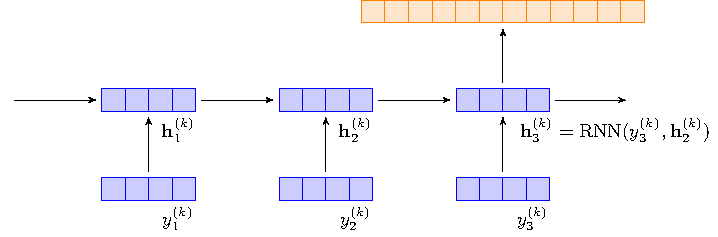
\includegraphics[scale=0.7]{rnntikzpicz/predrnnlm}
\end{center}


%\item Score of $t$'th word following history $y_{1:t-1}^{(k)}$:
\begin{align*}
s(w, \hat{y}_{1:t-1}^{(k)}) &= \only<1>{\ln p(\hat{y}^{(k)}_{1:t-1}| \boldx) + \ln \softmax(\mathbf{W}_{out} \, \mathbf{h}_{t-1}^{(k)} + \mathbf{b}_{out})}\only<2->{\tst{\ln p(\hat{y}^{(k)}_{1:t-1}| \boldx) + \ln \softmax(\mathbf{W}_{out} \, \mathbf{h}_{t-1}^{(k)} + \mathbf{b}_{out})}} \\
\only<2->{&= \mathbf{W}_{out} \, \mathbf{h}_{t-1}^{(k)} + \mathbf{b}_{out}}
\end{align*}

\air
\air
\only<3>{
\begin{itemize}
\item Can set $s(w, \hat{y}_{1:t-1}^{(k)}) \niceq {-}\infty$ if $(w, \hat{y}_{1:t-1}^{(k)})$ violates a hard constraint
\end{itemize}
}
\end{frame}

\begin{frame}[fragile]
\frametitle{Computing Gradients of the Loss ($K\niceq3$)}

    \begin{center}
    \air
    \air
    \air
    \air

  \begin{tikzpicture}[transform canvas = {scale=0.8}]
  \tikzstyle{beam}=[draw, minimum height=0.6cm, anchor=base, text height=5, text depth=0, minimum width=1.5cm,thin, rounded corners, line width=0.03cm]
  \tikzstyle{mat}=[draw=white]
\tikzset{>=stealth',every on chain/.append style={join},
         every join/.style={->}}

     
       % \node[draw = white, yshift=1.8cm]{Time Step};
       %\node[draw = white, xshift=-7.5cm, yshift=0.5cm]{Beam:};
       \begin{scope}
         

   \matrix (G) [matrix of nodes, nodes={beam},inner sep=1mm,row sep=0.03cm, column sep=0.8cm ] {
    \node<1->[fill=yellow](G-1-1){\textcolor{blue}{a}}; & \node<2->[fill=yellow](G-1-2){red}; & \node<3->[fill=lightgray](G-1-3){\textcolor{blue}{dog}}; & \node<4->(G-1-4){smells}; & \node<8->[fill=lightgray](G-1-5){\textcolor{red}{home}};  & \node<9->(G-1-6){{today}}; \\
    \node<1->(G-2-1){the}; & \node<2->(G-2-2){dog}; & \node<3->[fill=yellow](G-2-3){dog}; & \node<4->(G-2-4){barks}; & \node<8->[fill=yellow](G-2-5){quickly}; & \node<9->(G-2-6){Friday}; \\
    \node<1->(G-3-1){red}; & \node<2->[fill=lightgray](G-3-2){\textcolor{blue}{blue}}; & \node<3->(G-3-3){cat}; &  \node<4->[fill=lightgray](G-3-4){\textcolor{blue}{barks}}; & \node<8->(G-3-5){straight}; & \node<9->[fill=lightgray](G-3-6){\textcolor{red}{now}}; \\
    & & & \node<4->[fill=yellow](G-4-4){runs}; & & \node<9->[fill=yellow](G-4-6){today}; \\
    };

    \only<2->{
      \draw[->] (G-1-1.east) -> (G-1-2.west); 
      \draw[->] (G-2-1.east) -> (G-2-2.west); 
      \draw[->] (G-1-1.east) -> (G-3-2.west); 
      \draw[double, line width=0.03cm] (G-3-1.south west) -- (G-3-2.south east);
    }
  
    \only<3->{
      \draw[->] (G-1-2.east) -> (G-2-3.west); 
      \draw[->] (G-3-2.east) -> (G-3-3.west); 
      \draw[->] (G-3-2.east) -> (G-1-3.west); 
      \draw[double, line width=0.03cm] (G-3-1.south west) -- (G-3-3.south east);
    }
    
 \only<4->{
    \draw[->] (G-2-3.east) -> (G-4-4.west); 
    \draw[->] (G-1-3.east) -> (G-3-4.west); 
    \draw[->] (G-2-3.east) -> (G-2-4.west); 
    \draw[->] (G-1-3.east) -> (G-1-4.west); 
    \draw[double, line width=0.03cm] (G-3-1.south west) -- (G-3-4.south east);
}

 \only<9->{
    \draw[->] (G-1-5.east) -> (G-1-6.west); 
    \draw[->] (G-1-5.east) -> (G-3-6.west); 
    \draw[->] (G-2-5.east) -> (G-2-6.west); 
    \draw[->] (G-2-5.east) -> (G-4-6.west); 
    \draw[double, line width=0.03cm] (G-3-1.south west) -- (G-3-6.south east);
}

    % \draw[->] (G-3-2.east) -> (G-3-3.west); 
    % \draw[->] (G-3-2.east) -> (G-1-3.west); 

 \only<8->{
    \draw[->, dashed] (G-4-4.east) -> (G-1-5.west); 
    \draw[->, dashed] (G-4-4.east) -> (G-2-5.west); 
    \draw[->, dashed] (G-4-4.east) -> (G-3-5.west); 
    \draw[double, line width=0.03cm] (G-3-1.south west) -- (G-3-5.south east);
}

       \end{scope}
\end{tikzpicture}
  \end{center}  

  \air 
  \air 
  \air 
  \only<-4>{
 \begin{align*}
 \mathcal{L}&(\theta) = \sum_{t} \Delta(\hat{y}_{1:t}^{(K)}) \left[1  - s(y_t, y_{1:t-1}) + s(\hat{y}_t^{(K)}, \hat{y}_{1:t-1}^{(K)}) \right] 
\end{align*}}  
  \only<5->{
 \begin{align*}
 \mathcal{L}&(\theta) = \sum_{t} \Delta(\hat{y}_{1:t}^{(K)}) \left[1  - \colorbox{yellow}{\strut$s(y_t, y_{1:t-1})$} + \colorbox{lightgrey}{\strut$s(\hat{y}_t^{(K)}, \hat{y}_{1:t-1}^{(K)})$} \right] 
\end{align*}}

\only<-4>{
  \begin{itemize}
  \item Color \textcolor{yellow}{Gold}: target sequence $y$
  \air
  \item Color \textcolor{gray}{Gray}: violating sequence $\hat{y}^{(K)}$

\vspace*{0.7cm}
 \end{itemize}
}
\only<5-7>{
\begin{itemize}
  \item<5-> Need to BPTT for both $y_{1:t}$ and $\hat{y}_{1:t}^{(K)}$, which is $O(T)$
  \air
  \item<6-> Worst case: violation at each $t$ gives $O(T^2)$ backward pass
  \air
  \item<7-> \textbf{Idea:} use LaSO~\citep{daume05learning} beam-update
  \end{itemize}
}
\only<8->{
\vspace*{0.70cm}
\textbf{LaSO}~\citep{daume05learning}:
\begin{itemize}
\item  If no margin violation at $t\,{-}\,1$, update beam as usual
\air
\item Otherwise, update beam with sequences prefixed by $y_{1:t-1}$
\end{itemize}
}
%\centerline{Loss}
%  \vspace{-0.5cm}

\end{frame}

%\begin{frame}
%\frametitle{Efficiency Concerns}
%
%\begin{align*}
% \mathcal{L}&(\theta) = \sum_{t} \Delta(\hat{y}_{1:t}^{(K)}) \left[1 - \colorbox{yellow}{\strut$f(y_t, y_{1:t-1}, \boldx)$} +  \colorbox{lightgrey}{\strut$f(\hat{y}_t^{(K)}, \hat{y}_{1:t-1}^{(K)}, \boldx)$} \right] 
%\end{align*}
%
%\begin{itemize}
%\item Get gradients for gold sequence \textit{and} $K$'th sequence on the beam
%\air
%\item $\frac{\partial \mcL}{\partial f(y_{1:t})}$ and $\frac{\partial \mcL}{\partial f(\hat{y}_{1:t}^{(K)})}$ each require BPTT, which is $O(T)$
%\air
%\item Worst case: margin violation at each $t$ gives $O(T^2)$ for full backward pass
%\end{itemize}
%
%\end{frame}
%
%\begin{frame}
%\frametitle{Getting an $O(T)$ Backward Pass}
%\textbf{Idea:} use LaSO~\citep{daume05learning} search-update:
%\air
%\begin{itemize}
%\item If no margin violation at $t-1$, set beam at time $t$ as usual
%\air
%\item Otherwise, set beam at $t$ to contain \textit{only} sequences with $y_{1:t-1}$ as a prefix
%\end{itemize}
%\end{frame}

\begin{frame}[fragile]
  \frametitle{Backpropagation over Structure}
  \begin{center}
    
  \air 
  \air 
  \air 

  \begin{tikzpicture}[transform canvas = {scale=0.8}]
    \tikzstyle{beam}=[draw, minimum height=0.6cm, anchor=base, text height=5, text depth=0, minimum width=1.5cm,thin, rounded corners, line width=0.03cm]
    \tikzstyle{mat}=[draw=white]
    \tikzset{>=stealth',every on chain/.append style={join},
      every join/.style={->}}
    
     
       % \node[draw = white, yshift=1.8cm]{Time Step};
       %\node[draw = white, xshift=-7.5cm, yshift=0.5cm]{Beam:};
       \begin{scope}
         

   \matrix (G) [matrix of nodes, nodes={beam},inner sep=1mm,row sep=0.03cm, column sep=0.8cm ] {
     \node[fill=yellow](G-1-1){\textcolor{blue}{a}}; & \node[fill=yellow](G-1-2){red}; & \node[fill=lightgray](G-1-3){\textcolor{blue}{dog}}; & \node(G-1-4){smells}; & \node[fill=lightgray](G-1-5){\textcolor{red}{home}};  & \node(G-1-6){{today}}; \\
     \node(G-2-1){the}; & \node(G-2-2){dog}; & \node[fill=yellow](G-2-3){dog}; & \node(G-2-4){barks}; & \node[fill=yellow](G-2-5){quickly}; & \node(G-2-6){Friday}; \\
     \node(G-3-1){red}; & \node[fill=lightgray](G-3-2){\textcolor{blue}{blue}}; & \node(G-3-3){cat}; &  \node[fill=lightgray](G-3-4){\textcolor{blue}{barks}}; & \node(G-3-5){straight}; & \node[fill=lightgray](G-3-6){\textcolor{red}{now}}; \\
     & & & \node[fill=yellow](G-4-4){runs}; & & \node[fill=yellow](G-4-6){today}; \\
    };


    \draw[->] (G-1-1.east) -> (G-1-2.west); 
    \draw[->] (G-2-1.east) -> (G-2-2.west); 
    \draw[->] (G-1-1.east) -> (G-3-2.west); 
    \draw[double, line width=0.03cm] (G-3-1.south west) -- (G-3-2.south east);


    \draw[->] (G-1-2.east) -> (G-2-3.west); 
    \draw[->] (G-3-2.east) -> (G-3-3.west); 
    \draw[->] (G-3-2.east) -> (G-1-3.west); 
    \draw[double, line width=0.03cm] (G-3-1.south west) -- (G-3-3.south east);

    \draw[->] (G-2-3.east) -> (G-4-4.west); 
    \draw[->] (G-1-3.east) -> (G-3-4.west); 
    \draw[->] (G-2-3.east) -> (G-2-4.west); 
    \draw[->] (G-1-3.east) -> (G-1-4.west); 
    \draw[double, line width=0.03cm] (G-3-1.south west) -- (G-3-4.south east);

    \draw[->] (G-1-5.east) -> (G-1-6.west); 
    \draw[->] (G-1-5.east) -> (G-3-6.west); 
    \draw[->] (G-2-5.east) -> (G-2-6.west); 
    \draw[->] (G-2-5.east) -> (G-4-6.west); 
    \draw[double, line width=0.03cm] (G-3-1.south west) -- (G-3-6.south east);


    % \draw[->] (G-3-2.east) -> (G-3-3.west); 
    % \draw[->] (G-3-2.east) -> (G-1-3.west); 


    \draw[->, dashed] (G-4-4.east) -> (G-1-5.west); 
    \draw[->, dashed] (G-4-4.east) -> (G-2-5.west); 
    \draw[->, dashed] (G-4-4.east) -> (G-3-5.west); 
    \draw[double, line width=0.03cm] (G-3-1.south west) -- (G-3-5.south east);


       \end{scope}

       \begin{scope}[yshift=-2.8cm]

      \matrix (G) [matrix of nodes,nodes={beam}, inner sep=1mm,row sep=0.06cm,column sep=0.8cm ] {
        \node[fill=yellow](G-1-1){a}; & \node[fill=yellow](G-1-2){red}; & \node[fill=yellow](G-1-3){dog}; & \node[fill=yellow](G-1-4){runs}; & \node[fill=yellow](G-1-5){quickly}; & \node[fill=yellow](G-1-6){today}; \\
         & \node[fill=lightgray](G-2-2){\textcolor{blue}{blue}}; & \node[fill=lightgray](G-2-3){\textcolor{blue}{dog}}; & \node[fill=lightgray](G-2-4){\textcolor{blue}{barks}}; & \node[fill=lightgray](G-2-5){\textcolor{red}{home}}; & \node[fill=lightgray](G-2-6){\textcolor{red}{now}}; \\
      };
    \draw[->] (G-1-1.east) -> (G-1-2.west); 
    \draw[->] (G-1-2.east) -> (G-1-3.west); 
    \draw[->] (G-1-3.east) -> (G-1-4.west); 
    \draw[->] (G-1-4.east) -> (G-1-5.west); 
    \draw[->] (G-1-5.east) -> (G-1-6.west); 

    \draw[->] (G-1-1.east) -> (G-2-2.west); 
    \draw[->] (G-2-2.east) -> (G-2-3.west); 
    \draw[->] (G-2-3.east) -> (G-2-4.west); 
    \draw[->] (G-1-4.east) -> (G-2-5.west); 
    \draw[->] (G-2-5.east) -> (G-2-6.west); 
      
    \end{scope}
  \end{tikzpicture}  
  \end{center}
  \vspace{2cm}
  \vspace{1cm}
  
  \begin{itemize}
  \item Margin gradients are sparse, only violating sequences get updates.
  \item Backprop only requires 2x time as standard methods. 
  \end{itemize}
\end{frame}

%\begin{frame}
%\frametitle{LaSO-style Search (with Constraints)}
%
%\begin{enumerate}
%\item[(1)] Initialize (empty) beam of hypotheses $\hat{y}_{1:0}^{(1:K)}$
%\air
%\item[(2)] For $t \niceq 1 \ldots T$:
%   \begin{enumerate}
%   \item[(a)] Compute for all $k$ and all possible output words $w$:
%     \begin{align*}
%     \hspace*{-4cm} s(\hat{y}_t \niceq w, \hat{y}_{1:t-1}^{(k)}) \gets f(\hat{y}_t^{(k)} \niceq w, \hat{y}_{1:t-1}^{(k)})
%     \end{align*}
%   \item[(b)] Reset beam:
%\begin{align*}
%          \hat{y}_{1:t}^{(1:K)} \gets \topK_{s} \begin{cases}  \lbrace \mcV \times {y}_{1:t-1} \mid (w, y_{1:t-1}) \text{ valid } \rbrace &\mbox{violation at $t$} \\
%     \lbrace \mcV \times \hat{y}_{1:t-1}^{(1:K)} \mid (w, \hat{y}_{1:t-1}^{(k)}) \text{ valid } \rbrace &\mbox{otherwise} \end{cases}
%\end{align*} 
%\end{enumerate}
%\end{enumerate}
%\end{frame}

%\begin{frame}
%  \centerline{\structure{Related Work:} }
%  \air 
%  
%  % \pause
%
%  % Opinion: 
%  % \begin{itemize}
%  % \item 
%  %   DAD methods only address exposure bias, 
%  % \item RL is too strong a hammer .
%  % \end{itemize}
%
%  % \begin{itemize}
%  % \item 
%  % \end{itemize}
%\end{frame}

 \begin{frame}
   \frametitle{(Recent) Related Work and Discussion}
   \begin{itemize}
   \item Recent approaches to Exposure Bias, Label Bias:
  \begin{itemize}
  \item Data as Demonstrator, Scheduled Sampling \citep{Venkatraman,bengio15scheduled}
  \item Globally Normalized Transition-Based Networks \citep{Andor2016}
  \end{itemize}
  \air
  \item RL-based approaches
  \begin{itemize}
  \item MIXER \citep{ranzato16sequence}
  \item Actor-Critic \citep{Bahdanau2016}
  \end{itemize}
  \air
  \item Training with beam-search attempts to offer similar benefits
  \begin{itemize}
  \item Uses fact that we typically have gold prefixes in supervised text-generation to avoid RL
\end{itemize}   
\end{itemize}

%\begin{itemize}
%   \item Initial results are quite promising (but not yet SoTA)
%     \air
%   \item Results suggest RL may be unnecessary for these types of supervised tasks
%   \air
%   \item After all, in supervised text-generation we have gold prefixes!
%   \end{itemize}
 \end{frame}


\begin{frame}
  \frametitle{Experiments}
  \air 

  Experiments run on three Seq2Seq baseline tasks:

  \begin{itemize}
  \item Word Ordering, Dependency Parsing, Machine Translation
  \end{itemize}
  
\air
\air

We compare with Yoon Kim's implementation\footnote{\url{https://github.com/harvardnlp/seq2seq-attn}} of the Seq2Seq architecture of \Cite{Luong2015}.
\begin{itemize}
\item Uses LSTM encoders and decoders, attention, input feeding
%\item The beam-search variant (BSO) is identical, but without the output softmax
\item All models trained with Adagrad~\citep{duchi2011adaptive}
\item Pre-trained with NLL; $K$ increased gradually
\item ``BSO'' uses unconstrained search; ``ConBSO'' uses constraints
\end{itemize} 
 
\end{frame}


%\begin{frame}
%\frametitle{Getting Things to Work}
%\begin{align*}
% \mathcal{L}&(\theta) = \sum_{t} \Delta(\hat{y}_{1:t}^{(K)}) \left[1 - f(y_t, y_{1:t-1}, \boldx) +  f(\hat{y}_t^{(K)}, \hat{y}_{1:t-1}^{(K)}, \boldx) \right] 
%\end{align*}
%
%Note:
%\begin{itemize}
%\item Get gradients only when gold falls off the beam
%\begin{itemize}
%\item And only for 2 sequences
%\end{itemize}
%\item Smaller $K$ $\Rightarrow$ more violations $\Rightarrow$ more gradient updates
%\end{itemize}
%
%\air
%\air
%Therefore, we:
%\begin{itemize}
%\item Pre-train with (word-level) cross-entropy 
%\item Increase $K$ gradually
%\end{itemize}
%\end{frame}

\begin{frame}
\frametitle{Word Ordering Experiments}
\begin{table}
\small
  \centering
  \begin{tabular}{lccc}
    \toprule
     & \multicolumn{3}{c}{Word Ordering (BLEU) } \\ 
          & $K_{te}$ = 1 & \onslide<2->{$K_{te}$ = 5} & \onslide<3->{$K_{te}$ = 10} \\ 
    \midrule
    Seq2Seq & 25.2 & \onslide<2->{29.8} & \onslide<3->{31.0} \\
    BSO     & 28.0 & \onslide<2->{33.2} & \onslide<3->{34.3} \\
    ConBSO & \textbf{28.6} & \onslide<2->{\textbf{34.3}} & \onslide<3->{\textbf{34.5}} \\
%    \midrule
%    LSTM-LM & 15.4 &  - & 26.8 \\
    \bottomrule
  \end{tabular}
\end{table}

\begin{itemize}
\item Map shuffled sentence to correctly ordered sentence
%\begin{itemize}
%\item (Somewhat artificial)
%\end{itemize}
\item Same setup as \Cite{liu15transition}
%\item All models trained with $K_{tr} \niceq 6$ 
%\item ConBSO enforces constraint (viz., that target be a permutation of source) during training
\item BSO models trained with beam of size 6
\end{itemize}
\end{frame}

\begin{frame}
\frametitle{Dependency Parsing Experiments}
\begin{itemize}
\item[Source:] {\color{red}{Ms. Haag plays Elianti .}}
\item[Target:] {\color{blue}{Ms. Haag @L\_NN plays @L\_NSUBJ Elianti @R\_DOBJ . @R\_PUNCT}}
\end{itemize}

\begin{table}
  \small
  \centering
  %\hspace*{-0.3cm}
  \begin{tabular}{@{}l@{\hspace{4pt}}ccc}
    \toprule
    & \multicolumn{3}{c}{Dependency Parsing (UAS/LAS) } \\ 
          & $K_{te}$ = 1 & $K_{te}$ = 5 & $K_{te}$ = 10 \\ 
    \midrule
    Seq2Seq & \textbf{87.33/82.26} & 88.53/84.16 & 88.66/84.33\\
    BSO & 86.91/82.11 & 91.00/\textbf{87.18} & 91.17/\textbf{87.41} \\
    ConBSO & 85.11/79.32 & \textbf{91.25}/86.92 & \textbf{91.57}/87.26 \\
%    \midrule
%    Andor & 93.17/91.18 & - & - \\ 
    \bottomrule
  \end{tabular}
\end{table}

\air
\begin{itemize}
%\item Map from source words to source words interleaved with arc-standard reduce actions
\item BSO models trained with beam of size 6
\item Same setup and evaluation as \Cite{chen14fast}
\item Certainly not SOA, but reasonable for word-only, left-to-right model
\end{itemize}
\end{frame}

\begin{frame}
\frametitle{Machine Translation: Impact of Non-0/1 $\Delta$}
\begin{table}[t!]
  \centering
  \begin{tabular}{lccc}
    \toprule
    & \multicolumn{3}{c}{Machine Translation (BLEU)} \\ 
     &  $K_{te}$ = 1 & $K_{te}$ = 5 & $K_{te}$ = 10 \\ 
    \midrule
       $\Delta(\beampred{t}{k}) \niceq \mathbf{1}\{\text{margin violation}\}$ & 25.73  & 28.21 & 27.43  \\
    $\Delta(\beampred{t}{k}) \niceq 1 \,{-}\,\mathrm{SentBLEU}(\hat{y}_{r+1:t}^{({K})}, y_{r+1:t})$ & 25.99  & 28.45 & 27.58 \\          
    \bottomrule
  \end{tabular}
\end{table}
%\begin{itemize}
%\item $\Delta(\beampred{t}{k}) \niceq 1 \,{-}\,\mathrm{SentBLEU}(\hat{y}_{r+1:t}^{({K})}, y_{r+1:t})$ vs. $\Delta(\beampred{t}{k}) \niceq \mathbf{1}_{\{\text{violation}\}}$
%\end{itemize}
\begin{itemize}
\item IWSLT 2014, DE-EN, development set
\item BSO models trained with beam of size 6
\item Nothing to write home about, but nice that we can tune to metrics
\end{itemize}
\end{frame}

\begin{frame}
\frametitle{Machine Translation Experiments}
\begin{table}[t!]
  \small
  \centering
  \begin{tabular}{lccc}
    \toprule
    & \multicolumn{3}{c}{Machine Translation (BLEU) } \\ 
    &  $K_{te}$ = 1 & $K_{te}$ = 5 & $K_{te}$ = 10 \\ 
    \midrule
    Seq2Seq & 22.53 & 24.03 & 23.87 \\
    BSO & \textbf{23.83} & \textbf{26.36} & \textbf{25.48} \\
    \midrule
    \midrule
    \onslide<2->{NLL} & \onslide<2->{17.74} & \onslide<2->{20.10} & \onslide<2->{20.28}\\
    \onslide<2->{DAD~\citep{Venkatraman}} & \onslide<2->{20.12} & \onslide<2->{22.25} & \onslide<2->{22.40} \\ 
    \onslide<2->{MIXER/RL~\citep{ranzato16sequence}} & \onslide<2->{20.73} & \onslide<2->{21.81} & \onslide<2->{21.83} \\
    %}    
    \bottomrule
  \end{tabular}
\end{table}
\begin{itemize}
\item IWSLT 2014, DE-EN
\item BSO models trained with beam of size 6
\item $\Delta(\beampred{t}{k}) = 1 \,{-}\,\mathrm{SentBLEU}(\hat{y}_{r+1:t}^{({K})}, y_{r+1:t})$
\item<2-> Results in bottom sub-table from \Cite{ranzato16sequence}
%\begin{itemize}
%\item XENT
%\end{itemize}
\item<2-> Note similar improvements to MIXER
\end{itemize}
\end{frame}



\begin{frame}
\frametitle{Conclusion}
Introduced a variant of Seq2Seq and training procedure that:
\begin{itemize}
\air
\item Attempts to mitigate Label Bias and Exposure Bias
\air
\item Allows tuning to test-time metrics
\air
\item Allows training with hard constraints
\air
\item Doesn't require RL
\end{itemize}

\air
\air
\textbf{N.B.} Backprop through search is a thing now/again:
\begin{itemize}
\item One piece of the CCG parsing approach of Lee et al. (2016), an EMNLP 2016 Best Paper!
\end{itemize}
\end{frame}

\begin{frame}
\begin{center}
Thanks!
\end{center}
\end{frame}

\begin{frame}
\frametitle{Training with Different Beam Sizes}
\begin{table}
 \small
  \centering
  \begin{tabular}{lccc}
    \toprule
    & \multicolumn{3}{c}{Word Ordering Beam Size (BLEU) } \\ 
    &  $K_{te}$ = 1 & $K_{te}$ = 5 & $K_{te}$ = 10 \\ 
    \midrule
    $K_{tr}$ = 2 & 30.59 & 31.23 & 30.26 \\
    $K_{tr}$ = 6 & 28.20 & 34.22 & 34.67 \\
    $K_{tr}$ = 11 & 26.88 & 34.42 & 34.88 \\   
%    \midrule
%    seq2seq & 26.11 & 30.20 & 31.04 \\         
    \bottomrule
  \end{tabular}
\end{table}

\begin{itemize}
\item ConBSO model, development set results
\end{itemize}
\end{frame}


\begin{frame}
\frametitle{Pseudocode}

\vspace*{-5mm}
{\scriptsize
\begin{algorithm}[H]
  \scriptsize
  \begin{algorithmic}[1]
    \Procedure{BSO}{$\boldx, K_{tr}, \suk$}
    %\State{/*\textsc{Forward}*/}
    \State{Init empty storage $\hat{y}_{1:T}$ and $\hat{\boldh}_{1:T}$; init $S_1$}
    \State{$r \gets 0$; $violations \gets \{0\}$}
    \For{$t=1,\ldots,T$} \Comment{\parbox[t]{7.1cm}{\raggedright Forward}}
    \State{$K \niceq K_{tr}$ if $t \, {\neq} \,T$ else $\displaystyle \argmax_{k: \beampred{t}{k} \neq \goldpfx{t}} {\footnotesize f(\hat{y}_t^{(k)}, \hat{\boldh}_{t-1}^{(k)})}$}
    \If{$f(y_{t}, \boldh_{t-1}) < f(\hat{y}_t^{(K)},\hat{\boldh}_{t-1}^{(K)}) + 1$}  
    \State{$\hat{\boldh}_{r:t-1} \gets \hat{\boldh}^{(K)}_{r:t-1}$}
    \State{$\hat{y}_{r+1:t} \gets \hat{y}^{(K)}_{r+1:t}$}    
    \State{Add $t$ to $violations$; $r \gets t$}
    %\State{$r \gets t$}
    \State{$S_{t+1} \gets \topK(  \suk(\goldpfx{t}))$}
    \Else{}
    \State{$S_{t+1} \gets \topK( \bigcup_{k=1}^K \suk(\beampred{t}{k})) $}
    \EndIf{}
    
    \EndFor{}
    %\State{/*\textsc{Backward}*/}
    \State{$grad\_{\boldh_{T}} \gets \bzero$; $grad\_{\widehat{\boldh}_{T}} \gets \bzero$}
    \For{$t=T-1,\ldots,1$} \Comment{\parbox[t]{7.1cm}{\raggedright Backward}}
    \State{$grad\_{\boldh_t} \, {\gets} \, \BRNN(\nabla_{\boldh_t} \mcL_{t+1}, grad\_{\boldh_{t+1}})$
      }
    \State{$grad\_{\widehat{\boldh}_t} \, {\gets} \, 
    \BRNN(\nabla_{\widehat{\boldh}_t} \mcL_{t+1}, grad\_{\widehat{\boldh}_{t+1}})$
      }      

    \If{$t \, {-} \, 1 \in violations$}
    \State{$grad\_{\boldh_t} \gets grad\_{\boldh_t} + grad\_{\widehat{\boldh}_t}$}     
    \State{$grad\_{\widehat{\boldh}_t} \gets \bzero$ }
    \EndIf{}
    \EndFor{}
    \EndProcedure{}
  \end{algorithmic}
\end{algorithm}
  }
\end{frame}

%\begin{frame}[fragile]
%      \frametitle{Search Example ($K=3$)}
%
%    \begin{center}
%    \air
%    \air
%    \air
%    \air
%
%  \begin{tikzpicture}[transform canvas = {scale=0.8}]
%  \tikzstyle{beam}=[draw, minimum height=0.6cm, anchor=base, text height=5, text depth=0, minimum width=1.5cm,thin, rounded corners, line width=0.03cm]
%  \tikzstyle{mat}=[draw=white]
%\tikzset{>=stealth',every on chain/.append style={join},
%         every join/.style={->}}
%
%     
%       % \node[draw = white, yshift=1.8cm]{Time Step};
%       %\node[draw = white, xshift=-7.5cm, yshift=0.5cm]{Beam:};
%       \begin{scope}
%         
%
%   \matrix (G) [matrix of nodes, nodes={beam},inner sep=1mm,row sep=0.03cm, column sep=0.8cm ] {
%    \node<1->[fill=yellow](G-1-1){\textcolor{blue}{a}}; & \node<2->[fill=yellow](G-1-2){red}; & \node<3->[fill=lightgray](G-1-3){\textcolor{blue}{dog}}; & \node<4->(G-1-4){smells}; & \node<5->[fill=lightgray](G-1-5){\textcolor{red}{home}};  & \node<6->[fill=lightgray](G-1-6){\textcolor{red}{today}}; \\
%    \node<1->(G-2-1){the}; & \node<2->(G-2-2){dog}; & \node<3->[fill=yellow](G-2-3){dog}; & \node<4->(G-2-4){barks}; & \node<5->[fill=yellow](G-2-5){quickly}; & \node<6->(G-2-6){Friday}; \\
%    \node<1->(G-3-1){red}; & \node<2->[fill=lightgray](G-3-2){\textcolor{blue}{blue}}; & \node<3->(G-3-3){cat}; &  \node<4->[fill=lightgray](G-3-4){\textcolor{blue}{barks}}; & \node<5->(G-3-5){straight}; & \node<6->[](G-3-6){now}; \\
%    & & & \node<4->[fill=yellow](G-4-4){runs}; & & \node<6->[fill=yellow](G-4-6){today}; \\
%    };
%
%    \only<2->{
%      \draw[->] (G-1-1.east) -> (G-1-2.west); 
%      \draw[->] (G-2-1.east) -> (G-2-2.west); 
%      \draw[->] (G-1-1.east) -> (G-3-2.west); 
%      \draw[double, line width=0.03cm] (G-3-1.south west) -- (G-3-2.south east);
%    }
%  
%    \only<3->{
%      \draw[->] (G-1-2.east) -> (G-2-3.west); 
%      \draw[->] (G-3-2.east) -> (G-3-3.west); 
%      \draw[->] (G-3-2.east) -> (G-1-3.west); 
%      \draw[double, line width=0.03cm] (G-3-1.south west) -- (G-3-3.south east);
%    }
%    
% \only<4->{
%    \draw[->] (G-2-3.east) -> (G-4-4.west); 
%    \draw[->] (G-1-3.east) -> (G-3-4.west); 
%    \draw[->] (G-2-3.east) -> (G-2-4.west); 
%    \draw[->] (G-1-3.east) -> (G-1-4.west); 
%    \draw[double, line width=0.03cm] (G-3-1.south west) -- (G-3-4.south east);
%}
% \only<6->{
%    \draw[->] (G-1-5.east) -> (G-1-6.west); 
%    \draw[->] (G-1-5.east) -> (G-3-6.west); 
%    \draw[->] (G-2-5.east) -> (G-2-6.west); 
%    \draw[->] (G-2-5.east) -> (G-4-6.west); 
%    \draw[double, line width=0.03cm] (G-3-1.south west) -- (G-3-6.south east);
%}
%
%    % \draw[->] (G-3-2.east) -> (G-3-3.west); 
%    % \draw[->] (G-3-2.east) -> (G-1-3.west); 
%
% \only<5->{
%    \draw[->, dashed] (G-4-4.east) -> (G-1-5.west); 
%    \draw[->, dashed] (G-4-4.east) -> (G-2-5.west); 
%    \draw[->, dashed] (G-4-4.east) -> (G-3-5.west); 
%    \draw[double, line width=0.03cm] (G-3-1.south west) -- (G-3-5.south east);
%}
%
%       \end{scope}
%    % \draw(G-1-1.north east) rectangle (G-3-1.south west);
%    % \draw(G-1-2.north east) rectangle (G-3-2.south west);
%
%    % \begin{scope}[yshift=-2.8cm]
%
%    %   \matrix (G) [matrix of nodes,nodes={beam}, inner sep=1mm,row sep=0.06cm,column sep=0.8cm ] {
%    %     \node[fill=yellow](G-1-1){a}; & \node[fill=yellow](G-1-2){red}; & \node[fill=yellow](G-1-3){dog}; & \node[fill=yellow](G-1-4){runs}; & \node[fill=yellow](G-1-5){quickly}; & \node[fill=yellow](G-1-6){today}; \\
%    %      & \node[fill=lightgray](G-2-2){\textcolor{blue}{blue}}; & \node[fill=lightgray](G-2-3){\textcolor{blue}{dog}}; & \node[fill=lightgray](G-2-4){\textcolor{blue}{barks}}; & \node[fill=lightgray](G-2-5){\textcolor{red}{home}}; & \node[fill=lightgray](G-2-6){\textcolor{red}{today}}; \\
%    %   };
%    % \draw[->] (G-1-1.east) -> (G-1-2.west); 
%    % \draw[->] (G-1-2.east) -> (G-1-3.west); 
%    % \draw[->] (G-1-3.east) -> (G-1-4.west); 
%    % \draw[->] (G-1-4.east) -> (G-1-5.west); 
%    % \draw[->] (G-1-5.east) -> (G-1-6.west); 
%
%    % \draw[->] (G-1-1.east) -> (G-2-2.west); 
%    % \draw[->] (G-2-2.east) -> (G-2-3.west); 
%    % \draw[->] (G-2-3.east) -> (G-2-4.west); 
%    % \draw[->] (G-1-4.east) -> (G-2-5.west); 
%    % \draw[->] (G-2-5.east) -> (G-2-6.west); 
%      
%    % \end{scope}
%\end{tikzpicture}
%  \end{center}  
%
%  \air 
%  \air 
%% \begin{align*}
%%  \mathcal{L}&(\theta) = \sum_{t} \Delta(\wvec_{1:t}, \wvec_{1:t}^{(K)}) \left[1 - f(\wvec_t, \wvec_{1:t-1}, \cvec) +  f(\wvec_t^{(K)}, \wvec_{1:t-1}^{(K)}, \cvec) \right] 
%% \end{align*}
%
%  \begin{itemize}
%  \item Color \textcolor{yellow}{Gold}: target sequence $y$
%  \item Color \textcolor{gray}{Gray}: violating sequence $\hat{y}^{(K)}$
%  \end{itemize}
%
%  \air 
%%  \centerline{Violation Criterion}
%%  \vspace{-0.5cm}
%%\begin{align*}
%% \mathcal{L}&(\theta) = \sum_{t} \Delta(y_{1:t}, \wvec_{1:t}^{K}) \left[1 - f(y_t, y_{1:t-1}, \cvec) +  f(\wvec_t^{(K)}, \wvec_{1:t-1}^{(K)}, \cvec) \right] 
%%\end{align*}
%
%\end{frame}

\begin{frame}[fragile]
  \frametitle{Backpropagation over Structure}
  \begin{center}
    
  \air 
  \air 
  \air 

  \begin{tikzpicture}[transform canvas = {scale=0.8}]
    \tikzstyle{beam}=[draw, minimum height=0.6cm, anchor=base, text height=5, text depth=0, minimum width=1.5cm,thin, rounded corners, line width=0.03cm]
    \tikzstyle{mat}=[draw=white]
    \tikzset{>=stealth',every on chain/.append style={join},
      every join/.style={->}}
    
     
       % \node[draw = white, yshift=1.8cm]{Time Step};
       %\node[draw = white, xshift=-7.5cm, yshift=0.5cm]{Beam:};
       \begin{scope}
         

   \matrix (G) [matrix of nodes, nodes={beam},inner sep=1mm,row sep=0.03cm, column sep=0.8cm ] {
     \node[fill=yellow](G-1-1){\textcolor{blue}{a}}; & \node[fill=yellow](G-1-2){red}; & \node[fill=lightgray](G-1-3){\textcolor{blue}{dog}}; & \node(G-1-4){smells}; & \node[fill=lightgray](G-1-5){\textcolor{red}{home}};  & \node[fill=lightgray](G-1-6){\textcolor{red}{today}}; \\
     \node(G-2-1){the}; & \node(G-2-2){dog}; & \node[fill=yellow](G-2-3){dog}; & \node(G-2-4){barks}; & \node[fill=yellow](G-2-5){quickly}; & \node(G-2-6){Friday}; \\
     \node(G-3-1){red}; & \node[fill=lightgray](G-3-2){\textcolor{blue}{blue}}; & \node(G-3-3){cat}; &  \node[fill=lightgray](G-3-4){\textcolor{blue}{barks}}; & \node(G-3-5){straight}; & \node[](G-3-6){now}; \\
     & & & \node[fill=yellow](G-4-4){runs}; & & \node[fill=yellow](G-4-6){today}; \\
    };


    \draw[->] (G-1-1.east) -> (G-1-2.west); 
    \draw[->] (G-2-1.east) -> (G-2-2.west); 
    \draw[->] (G-1-1.east) -> (G-3-2.west); 
    \draw[double, line width=0.03cm] (G-3-1.south west) -- (G-3-2.south east);


    \draw[->] (G-1-2.east) -> (G-2-3.west); 
    \draw[->] (G-3-2.east) -> (G-3-3.west); 
    \draw[->] (G-3-2.east) -> (G-1-3.west); 
    \draw[double, line width=0.03cm] (G-3-1.south west) -- (G-3-3.south east);

    \draw[->] (G-2-3.east) -> (G-4-4.west); 
    \draw[->] (G-1-3.east) -> (G-3-4.west); 
    \draw[->] (G-2-3.east) -> (G-2-4.west); 
    \draw[->] (G-1-3.east) -> (G-1-4.west); 
    \draw[double, line width=0.03cm] (G-3-1.south west) -- (G-3-4.south east);

    \draw[->] (G-1-5.east) -> (G-1-6.west); 
    \draw[->] (G-1-5.east) -> (G-3-6.west); 
    \draw[->] (G-2-5.east) -> (G-2-6.west); 
    \draw[->] (G-2-5.east) -> (G-4-6.west); 
    \draw[double, line width=0.03cm] (G-3-1.south west) -- (G-3-6.south east);


    % \draw[->] (G-3-2.east) -> (G-3-3.west); 
    % \draw[->] (G-3-2.east) -> (G-1-3.west); 


    \draw[->, dashed] (G-4-4.east) -> (G-1-5.west); 
    \draw[->, dashed] (G-4-4.east) -> (G-2-5.west); 
    \draw[->, dashed] (G-4-4.east) -> (G-3-5.west); 
    \draw[double, line width=0.03cm] (G-3-1.south west) -- (G-3-5.south east);


       \end{scope}

       \begin{scope}[yshift=-2.8cm]

      \matrix (G) [matrix of nodes,nodes={beam}, inner sep=1mm,row sep=0.06cm,column sep=0.8cm ] {
        \node[fill=yellow](G-1-1){a}; & \node[fill=yellow](G-1-2){red}; & \node[fill=yellow](G-1-3){dog}; & \node[fill=yellow](G-1-4){runs}; & \node[fill=yellow](G-1-5){quickly}; & \node[fill=yellow](G-1-6){today}; \\
         & \node[fill=lightgray](G-2-2){\textcolor{blue}{blue}}; & \node[fill=lightgray](G-2-3){\textcolor{blue}{dog}}; & \node[fill=lightgray](G-2-4){\textcolor{blue}{barks}}; & \node[fill=lightgray](G-2-5){\textcolor{red}{home}}; & \node[fill=lightgray](G-2-6){\textcolor{red}{today}}; \\
      };
    \draw[->] (G-1-1.east) -> (G-1-2.west); 
    \draw[->] (G-1-2.east) -> (G-1-3.west); 
    \draw[->] (G-1-3.east) -> (G-1-4.west); 
    \draw[->] (G-1-4.east) -> (G-1-5.west); 
    \draw[->] (G-1-5.east) -> (G-1-6.west); 

    \draw[->] (G-1-1.east) -> (G-2-2.west); 
    \draw[->] (G-2-2.east) -> (G-2-3.west); 
    \draw[->] (G-2-3.east) -> (G-2-4.west); 
    \draw[->] (G-1-4.east) -> (G-2-5.west); 
    \draw[->] (G-2-5.east) -> (G-2-6.west); 
      
    \end{scope}
  \end{tikzpicture}  
  \end{center}
  \vspace{2cm}
  \vspace{1cm}
  
  \begin{itemize}
  \item Margin gradients are sparse, only violating sequences get updates.
  \item Backprop only requires 2x time as standard methods. 
  \end{itemize}
\end{frame}

%\begin{frame}
%\frametitle{}
%Timing
%\end{frame}

\bibliographystyle{plainnat}
\bibliography{corefslides,full,master,seq2seqapps,ourwork,beamtrain}
\end{document}
